\subsection{Dos ejemplos de Integrales de Riemann}

Ahora, vamos a hacer un paréntesis para revisar dos ejemplos de integrales de Riemann.

\begin{ejem}
    Miremos la función $f(x) = x^3$ en el intervalo $[0,\alpha]$ con $\alpha > 0$.
\end{ejem}
    
\begin{marginfigure}
        \centering
        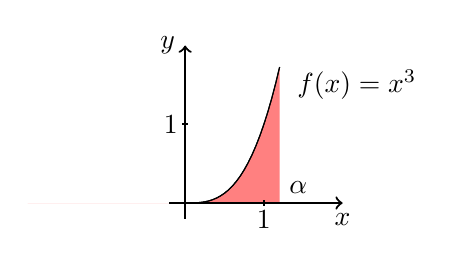
\begin{tikzpicture}
        
            \fill [red!50, domain=0:1.2, variable=\x]
              (-2, 0)
              -- plot ({\x}, {\x*\x*\x})
              -- (1.2, 0)
              -- cycle;
        
            \draw [thick] [->] (-0.2,0)--(2,0) node[right, below] {$x$};
             \foreach \x in {1,...,1}
               \draw[xshift=\x cm, thick] (0pt,-1pt)--(0pt,1pt) node[below] {$\x$};
        
            \draw [thick] [->] (0,-0.2)--(0,2) node[above, left] {$y$};
             \foreach \y in {1,...,1}
               \draw[yshift=\y cm, thick] (-1pt,0pt)--(1pt,0pt) node[left] {$\y$};
            
            \draw [domain=0:1.2, variable=\x]
              plot ({\x}, {\x*\x*\x}) node[right] at (1.3,1.5) {$f(x)=x^3$};
              
            \draw [domain=0:1.2, variable=\x]
              plot ({\x}, {\x*\x*\x}) node[right] at (1.2,0.2) {$\alpha$};
        \end{tikzpicture}
        \caption{\footnotesize Gráfica de $f(x) = x^3$.}
        \label{fig:ej1}
\end{marginfigure}
    
Lo que queremos es calcular el área sombreada en rojo como se ve en la figura \ref{fig:ej1} utilizando las sumas de Riemann.
    
En primer lugar, consideremos la partición canónica $P_n = \{ x_j \}_{j=0}^n$, donde $x_j = \frac{\alpha j}{n}$, y nuestros intervalos tendrán longitud $|I_j| = \alpha/n$.

Luego, sabemos que por definición $L(f,P_n)$ queda como

\[
L(f,P_n) = \sum_{j=1}^n m(f,P_n)|I_j| = \sum_{j=1}^n \frac{\alpha^3(j-1)^3}{n^3} \cdot \frac{\alpha}{n} \quad \footnotemark
\]\footnotetext{Recordemos que $m(f,P_n) = \frac{\alpha^3(j-1)^3}{n^3}$ para $j=1,\dots,n$ debido a que estamos tomando la función $x^3$, y cada subintervalo de $P_n$ está definido como $[\alpha(j-1)/n, \alpha j/n]$.}

\noindent y desarrollando este factor, nos queda

\[
\sum_{j=1}^n \frac{\alpha^3(j-1)^3}{n^3} \cdot \frac{\alpha}{n} = \frac{\alpha^4}{n^4} \sum_{j=1}^n (j-1)^3
\]

\noindent finalmente

\begin{equation}\label{eq:x^3}
L(f, P_n) = \frac{\alpha^4}{n^4} \frac{n^2(n-1)^2}{4} = \frac{\alpha^4}{n^2}\frac{(n-1)^2}{4} \quad \footnotemark
\end{equation}\footnotetext{Esto sale por el resultado de la siguiente suma:
\[
\sum_{j=1}^n j = \frac{n^2(n+1)^2}{4}
\]
Este resultado es demostrable a través de un argumento inductivo.}

Ahora, cuando $n \to \infty$, la igualdad \ref{eq:x^3}  nos queda como

\[
\lim_{n \to \infty} L(f,P_n) = \frac{\alpha^4}{4} \frac{(n-1)^2}{n^2} = \frac{\alpha^4}{4}
\]

Análogamente, tenemos que para $U(f, P_n)$

\[
U(f, P_n) = \sum_{j=1}^n \frac{\alpha^3 j^3}{n^3} \cdot \frac{\alpha}{n} = \frac{\alpha^4}{n^4} \sum_{j=1}^n j^3 = \frac{\alpha^4}{n^4}\frac{(n)^2(n+1)^2}{4}
\]

\noindent y el límite queda como

\[
\lim_{n \to \infty} U(f,P_n) = \frac{\alpha^4}{4} \frac{(n+1)^2}{n^2} = \frac{\alpha^4}{4}
\]

Como hemos llegado a que $U(f,P_n) = L(f,P_n) = \frac{\alpha^4}{4}$, entonces $f$ es integrable y más aún, $\int_0^{\alpha} x^3 = \frac{\alpha^4}{4}$.

\begin{ejem}
    Sea $f:[-1,1] \rightarrow \R$ definida de la siguiente manera:
    
    \[
    f(x) =
    \begin{cases}
    1 &\quad x = 0 \\
    \frac{1}{x^2} &\quad x\neq0
    \end{cases} 
    \]
\end{ejem}

\begin{marginfigure}
    \centering
    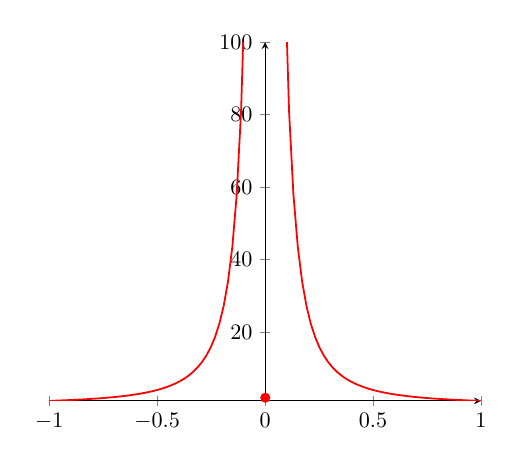
\begin{tikzpicture}[scale=0.8]
        \begin{axis}[
            xmin=-1,
            ymax=100,
            domain=-1:1,
            samples=100,
            axis y line=middle,
            axis x line=bottom,
            ]
            \addplot [red, thick] ({\x},{1/((\x)*(\x))});
        \end{axis}
    \filldraw [red] (3.43,0.05) circle (2pt);
    \end{tikzpicture}
    \caption{\footnotesize Gráfica de $f(x)$ sobre el intervalo $[1,1]$.}
    \label{fig:ej2}
\end{marginfigure}

Esta función no será integrable en el sentido de Riemann. En un principio, ya que la función es par y el intervalo de inegración es simétrico alrededor del 0, tenemos que

\[
\int_1^1 f(x)dx = 2\int_0^1 f(x)dx
\]

\noindent entonces, podemos centrarnos a calcular $\int_0^1 f(x)dx$. Esto sabemos que equivale a $\lim_{n \to \infty} L(f, P_n)$. Al ver a que equivale esas sumas inferiores con respecto a la partición canónica, tendremos que

\[
\lim_{n \to \infty} L(f, P_n) = \lim_{n \to \infty} \sum_{j=1}^n m_j|I_j|
\]

\noindent como la función es positiva, podemos estimar por arriba, luego

\[
\lim_{n \to \infty} \sum_{j=1}^n m_j|I_j| \geq \lim_{n \to \infty} m_{j_0}|I_{j_0}|
\]

\noindent entonces tenemos

\[
\lim_{n \to \infty} L(f, P_n) \geq \lim_{n \to \infty} \frac{2}{n} \frac{n^2}{4} = \infty
\]

De esta forma, la función no es Riemann-integrable.

\subsection{Propiedades y álgebra de las funciones integrables}

En primer lugar, veremos dos teoremas sobre integrabilidad que continuan desarrollando la idea de integrabilidad-continuidad que veníamos desarrollando desde el útlimo teorema enunciado.

\begin{teo}
    Sea $f: [a,b] \rightarrow \R$ acotada. Supongamos $f$ continua salvo en $x=c$. Entonces $f \in \Rint$\marginfootnote{La integrabilidad de la función no se ve afectada por ser discontinua en una cantidad finita de puntos.}.
\end{teo}

 \noindent\textit{Demostración.} Primero, como $f$ está acotada, entonces $\exists M>0$ tal que $|f(x)|<M$ para todo $x \in [a,b]$. A partir de este $M$, podemos establecer que dado $\varepsilon > 0$, escogemos $\delta >0$ tal que
    
\[
2M\delta < \frac{\varepsilon}{3}
\]
    
\noindent la existencia de dicho $\delta$ está garantizada por el lema de Arquímedes\marginfootnote{El lema de Arquímedes, o la propiedad arquimediana, se enuncia de la siguiente manera:
    
\begin{teo}
Sea $x > 0$, e $y$ un número real cualquiera, entonces existe un entero positivo $n$ tal que $nx > y$.
\end{teo}}. Ahora nos queda verificar que la función $f$ satisface la condición de Riemann:
    
\begin{marginfigure}
    \begin{tikzpicture}[x=70]
       \draw (-0.2,0) -- (2.2,0);      
       \draw (0, 0) node[below=7pt] {$a$};
       \draw[] (0,-0.1) -- (0,0.1);
       \draw[] (0.8,-0.1) -- (0.8,0.1);
       \draw (1, 0) node[below=7pt] {\ul{$c$}};
       \draw[] (1,-0.1) -- (1,0.1);
       \draw[decorate, decoration = {calligraphic brace, raise=5pt, amplitude=5pt}] (0,0.1) --  (0.8,0.1) node[pos=0.5,above=10pt,black]{$[a,c-\delta]$};
       \draw[decorate, decoration = {calligraphic brace, raise=5pt, amplitude=5pt}] (1.2,0.1) --  (2,0.1) node[pos=0.5,above=10pt,black]{$[c+\delta,b]$};
       \draw[] (1.2,-0.1) -- (1.2,0.1);
       \draw (2, 0) node[below=7pt] {$b$};
       \draw[] (2,-0.1) -- (2,0.1);
       \draw[>={Parenthesis[width=4mm,line width=1pt,length=1.5mm]},<->] (0.8, 0) -- (1.2, 0);
    \end{tikzpicture}
    \caption{\footnotesize Representación gráfica de los intervalos descritos en la demostración.}
    \label{fig:int1}
\end{marginfigure}

Como se ve en la figura \ref{fig:int1}, en el intervalo $[a,b]$ construiremos dos intervalos alrededor de $c$: Uno será $[a,c-\delta]$ y el otro $[c+\delta,b]$, en los cuales sabemos que la función es continua y acotada, luego definamos dos particiones $P_1$ y $P_2$, ambas dependientes de $\varepsilon$, y definidas sobre $[a,c-\delta]$ y $[c+\delta,b]$ respectivamente. Por ser la función $f$ continua y acotada dentro de estos intervalos, entonces $P_1$ y $P_2$ satisfacerán la condición de Riemann \ref{teo:condrie}, por lo que $f$ es integrable dentro de estos intervalos.

Ahora, lo que nos queda es preguntarnos qué sucede en el intervalo que contiene al punto $c$. Entonces, sea $\Delta_0 = [c-\delta, c+\delta]$, tenemos que

\[
\big( M(f, \Delta_0) - m(f, \Delta_0) \big)|\Delta_0| \leq 2M\delta < \frac{\varepsilon}{3} \quad \footnotemark
\]\footnotetext{Recordemos que $f(x)$ está acotada, por lo tanto $M(f, \Delta_0) < M$ y $m(f, \Delta_0) < M$, y esta desigualdad sale por desigualdad triangular. Y además, $|\Delta_0| = \delta$ por como se construyó el intervalo.}

Por otro lado, como $f$ es continua en $[a,c-\delta]$ y en $[c+\delta,b]$, entonces existen $P_1$, $P_2$ dependientes de $\varepsilon$ tales que

\[
U(f, P_1) - L(f,P_1) < \frac{\varepsilon}{3}, \quad U(f, P_2) - L(f,P_2) < \frac{\varepsilon}{3}
\]

Definamos ahora $\Pe = P_1 \cup P_2 \cup \{c-\delta, c+\delta\}$, entonces

\[
U(f, \Pe) - L(f, \Pe) \leq \varepsilon
\]

\noindent esto implica que la función completa, incluyendo el intervalo donde se encuentra el punto $c$, es integrable. Por lo que el teorema queda demostrado
\qed

\begin{teo}
    Si $f \equiv 0$ salvo en $x = c$ entonces $f \in \Rint$\marginfootnote{Este resultado se puede generalizar utilizando un argumento inductivo.}.
\end{teo}

\begin{proof}
    Tomemos una partición $P_n = \{ x_j \}_{j=0}^n$ (con $n \in \N$), tal que dado $\varepsilon > 0$,
    
    \[
    |f(c)|\frac{(b-a)}{n} < \varepsilon
    \]
    
    Como la función vale cero en todo el intervalo $[a,b]$, excepto en un punto $c$, tendremos que
    
    \[
    U(f, P_n) = M(f, I_{j_0})|I_{j_0}|, \quad L(f, P_n) = m(f, I_{j_0})|I_{j_0}|
    \]
    
    \noindent donde $I_{j_0}$ es el subintervalo que contiene a $c$. Si $c$ se encontrase en uno de los extremos, bastaría con refinar la partición $P_n$ hasta que quede dentro de algún $I_j$.
    
    Entonces, al tomar la diferencia de las sumas inferiores y superiores,
    
    \[
    U(f,P_n) - L(f,P_n) \leq |f(c)|\frac{(b-a)}{n} < \varepsilon
    \]
    
    \noindent por lo tanto, $f \in \Rint$.
    
    Más aún, como comentario adicional, se puede deducir que $\intab f(x)dx = 0$.
\end{proof}